%%%%%%%%%%%%%%%%%%%%%%%%%%%%%%%%%%%%%%%%%%%%%%%%%%%%%%
% A Beamer template for Ritsumeikan University       %
% Author: Ming-Hao Xu (Xu Minghao)                   %
% Date:   April 2022.                                %
% LPPL Licensed.                                     %
%%%%%%%%%%%%%%%%%%%%%%%%%%%%%%%%%%%%%%%%%%%%%%%%%%%%%%

\documentclass[10pt]{beamer}
\usepackage{hyperref}

\usepackage[UTF8]{ctex}
\usepackage[T1]{fontenc}
\usepackage[backend=bibtex]{biblatex}
\addbibresource{ref.bib}

% other packages
\usepackage{latexsym,amsmath,xcolor,multicol,booktabs,calligra}
\usepackage{graphicx,pstricks,listings,stackengine,multirow}
\usefonttheme[onlymath]{serif}

\usepackage{tikz}
\usetikzlibrary{
  arrows.meta,
  calc,
  fit,
  positioning,
  quotes,
  fadings
}
\tikzset{>=latex}

\usepackage{algorithm}
\usepackage{caption}
\usepackage{algorithmicx}
\usepackage{algpseudocode}
\usepackage{bbm}
\floatname{algorithm}{Algorithm} %算法
\renewcommand{\algorithmicrequire}{\textbf{Input:}} %输入
\renewcommand{\algorithmicensure}{\textbf{Output:}} %输出

\captionsetup[figure]{labelfont={bf},labelformat={default},labelsep=period,name={Fig.}}

% dummy text; remove it when working on this template
\usepackage{lipsum}

\setbeamerfont{footnote}{size=\tiny}

\author{Wenchong Huang}
\title{Optimal Transport}
\subtitle{Theory, Computation and Applications}
\institute{
    School of Mathematical Sciences, \\
    Zhejiang University.
}
\date{Dec. 30th, 2024}
\usepackage{Ritsumeikan}

% defs
\def\cmd#1{\texttt{\color{red}\footnotesize $\backslash$#1}}
\def\env#1{\texttt{\color{blue}\footnotesize #1}}
\definecolor{deepblue}{rgb}{0,0,0.5}
\definecolor{deepred}{rgb}{0.6,0,0}
\definecolor{deepgreen}{rgb}{0,0.5,0}
\definecolor{halfgray}{gray}{0.55}

\lstset{
    basicstyle=\ttfamily\tiny,
    keywordstyle=\bfseries\color{deepblue},
    emphstyle=\ttfamily\color{deepred},    % Custom highlighting style
    stringstyle=\color{deepgreen},
    numbers=left,
    numberstyle=\small\color{halfgray},
    rulesepcolor=\color{red!20!green!20!blue!20},
    frame=shadowbox,
}

\newcommand{\R}{\mathbb{R}}
\newcommand{\mX}{\mathcal{X}}
\newcommand{\mY}{\mathcal{Y}}
\newcommand{\mL}{\mathcal{L}}
\newcommand{\wass}{\mathcal{W}}
\newcommand{\pbms}{\mathcal{M}_+^1(\mX)}
\newcommand{\pbmsy}{\mathcal{M}_+^1(\mY)}
\newcommand{\cfun}{\mathcal{C}(\mX)}
\newcommand{\cfuny}{\mathcal{C}(\mY)}

\newtheorem{Def}{\textbf{Definition}}[section]
\newtheorem{Thm}{\textbf{Theorem}}[section]
\newtheorem{Exm}{\textbf{Example}}[section]

\begin{document}

\begin{frame}
    \titlepage
\end{frame}

\begin{frame}{Overview}
    \scriptsize
    \vspace{-1.5em}
    \begin{figure}
        \captionsetup{font=tiny}
        \begin{minipage}[t]{0.6\linewidth}
            \vspace{0pt}
            \textbf{Principal concern:} the distance between two probability measures.

            \textbf{First introduced} in 1781 by Monge.

            \textbf{Relative subjects:} probability theory, geometry, graph theory, machine learning...

            \textbf{Applications:}
            \begin{itemize}
                \item Image registration and warping;
                \item Reflector design;
                \item Retrieving information from shadowgraphy and proton radiography;
                \item Seismic tomography and reflection seismology.
            \end{itemize}

            \textbf{Some well-known researchers:}
            \begin{itemize}
                \item Gasoard Monge (France);
                \item Leonid Kantorovich (Russia);
                \item Yann Brenier (France);
                \item Xianfeng Gu (顾险峰, China);
            \end{itemize}
            \centering
            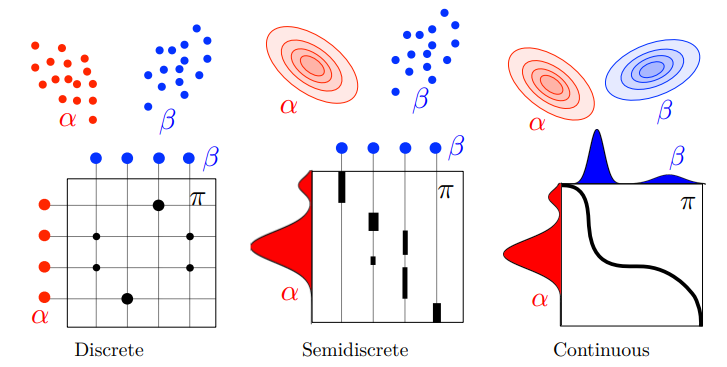
\includegraphics[width=0.6\textwidth]{png/3TypesOfOT.png}
            \vspace{-.7em}
            \caption{Three main scenarios for Kantorovich OT}
        \end{minipage}
        \begin{minipage}[t]{0.38\linewidth}
            \vspace{0pt}
            \centering
            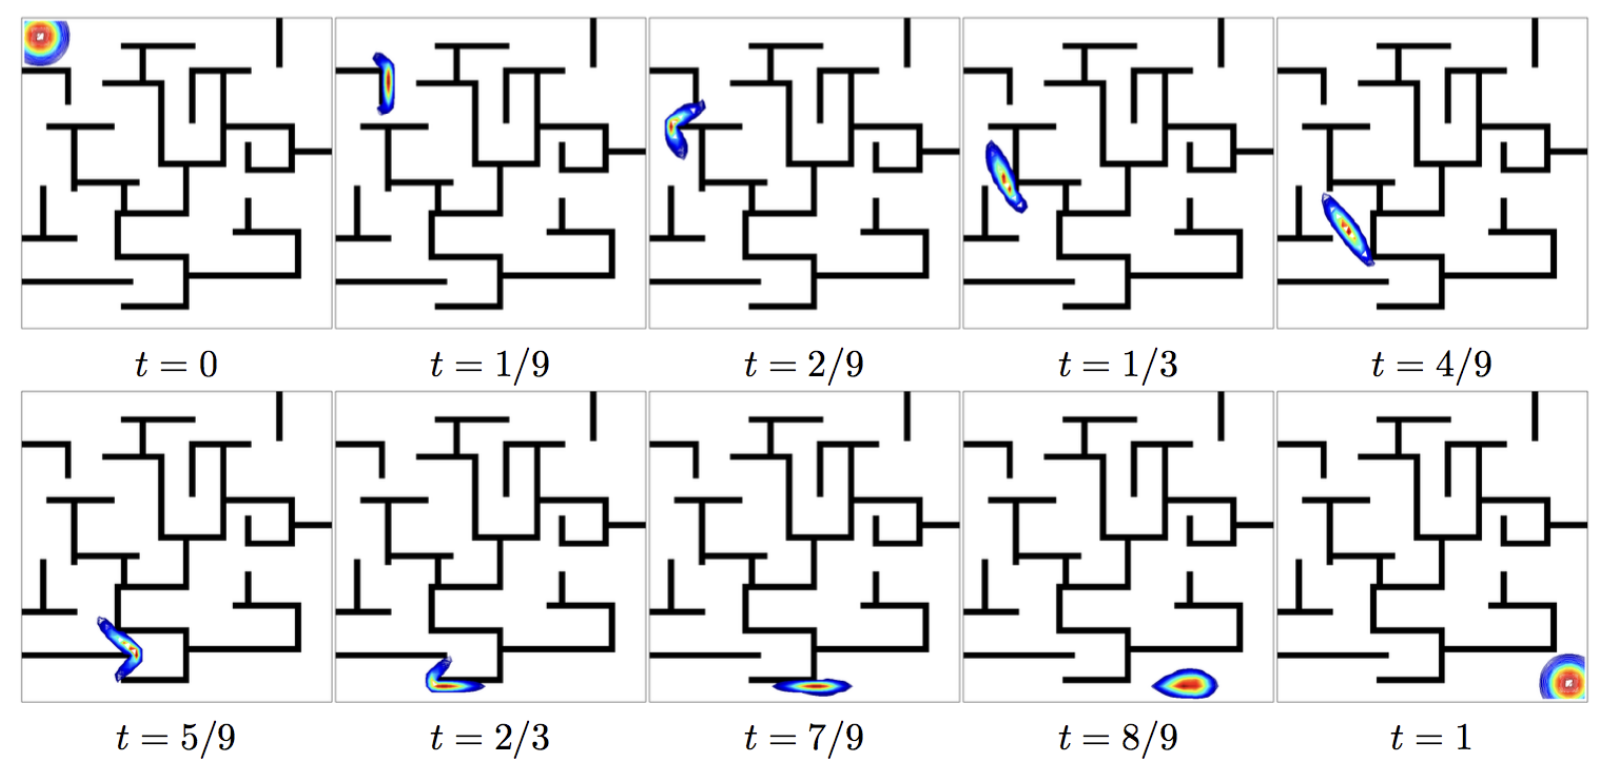
\includegraphics[width=0.98\textwidth]{png/maze.png}
            \caption{Solving maze with OT}
            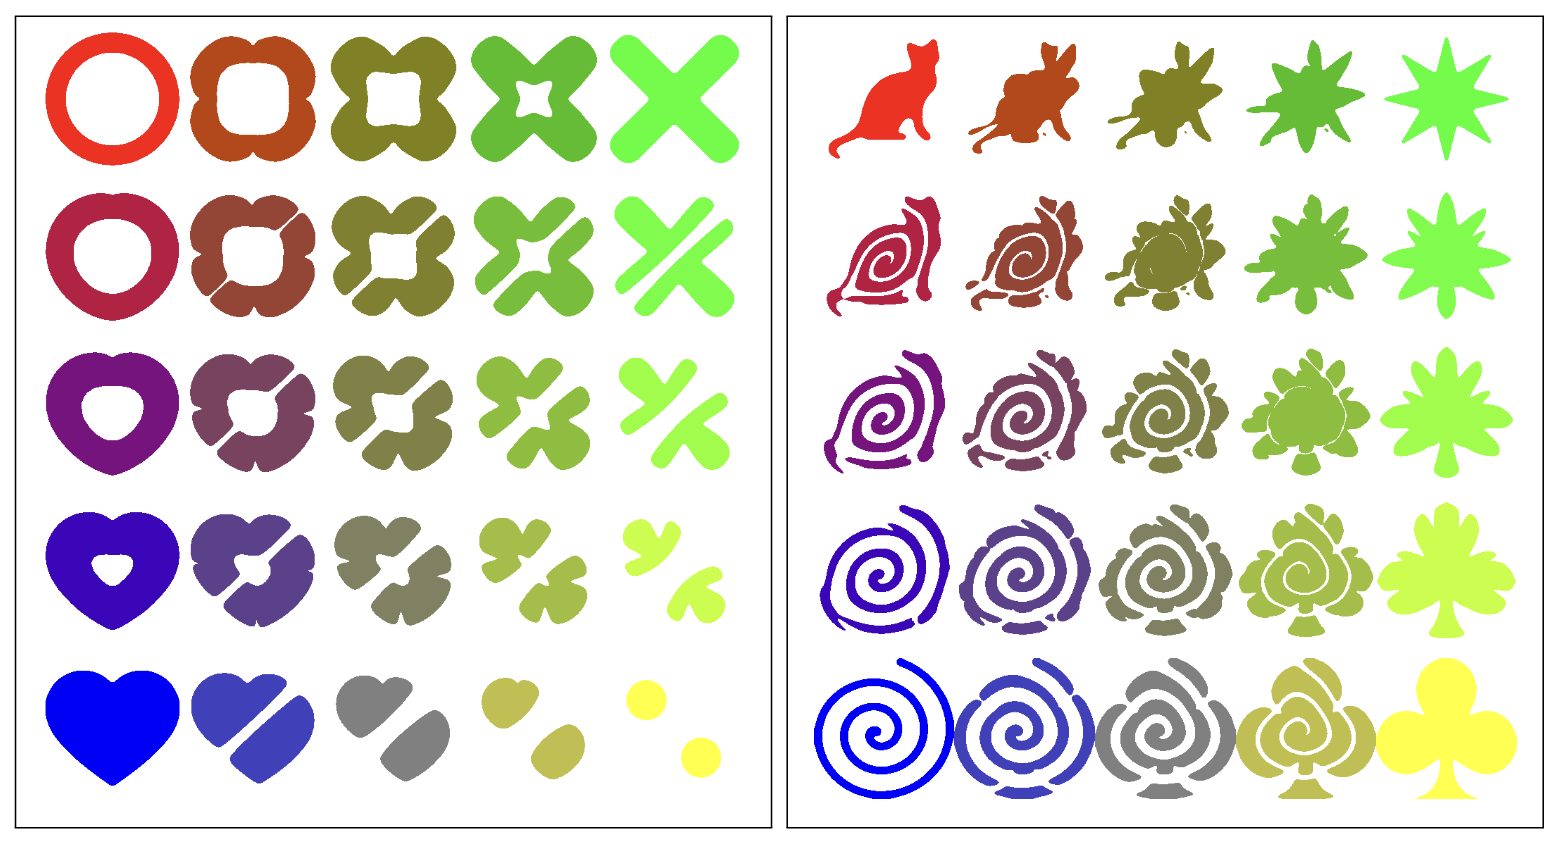
\includegraphics[width=0.98\textwidth]{png/2DShapeInterpolation.png}
            \caption{2D shape interpolation with OT}
            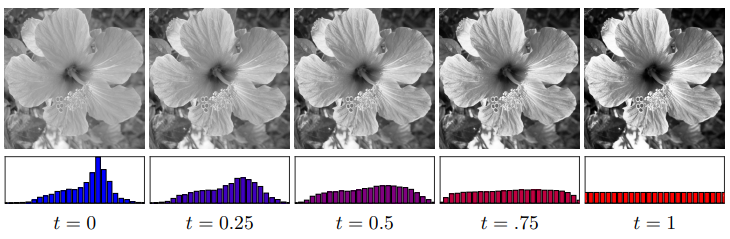
\includegraphics[width=0.98\textwidth]{png/HistogramEqualization.png}
            \caption{Histogram equalization with OT}
        \end{minipage}
    \end{figure}
\end{frame}

\section{Theory}

\begin{frame}{The sand-moving problem}
    \footnotesize
    A child wants to make a pile of sand in the shape of a castle.

    \textbf{Cost:} 1 kcal per shovel and per meter horizontally.

    \textbf{Target:} Minimize the total cost.

    \begin{figure}
        \captionsetup{font=scriptsize}
        \centering
        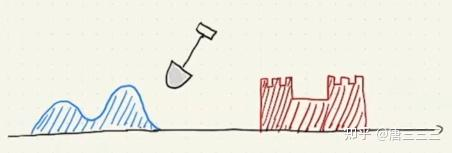
\includegraphics[width=0.8\textwidth]{png/SandMoving.jpg}
        \caption{The sand-moving problem.}
    \end{figure}

    \pause
    Let's denote the source shape by $f(x)$ and the target by $g(x)$. 
    The sand-moving problem cound be formulated as: 
    find a \textbf{transport mapping} $T:\R\to\R$ to minimize
    \begin{equation}
        \int_{\R} |T(x)-x|f(x)\;dx,
    \end{equation}
    which satisfies
    \begin{equation}
        \int_{T(U)} g(x)\;dx = \int_{U} f(x)\;dx\; \text{for all open interval}\; U\subset\R.
    \end{equation}
\end{frame}

\begin{frame}{The allocation problem}
    \footnotesize
    There are some steel coils to be transported from warehouses to factories.
    The transport cost is \$1 per coil and per kilometer.
    How to minimize the total cost?

    \begin{figure}
        \captionsetup{font=scriptsize}
        \centering
        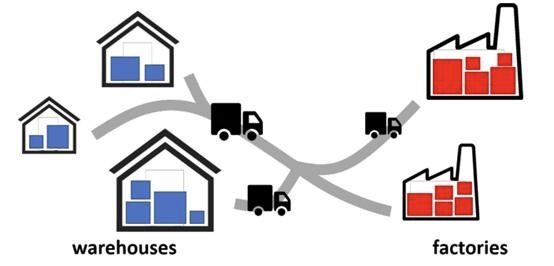
\includegraphics[width=0.6\textwidth]{png/SteelTransport.jpg}
        \caption{The allocation problem.}
    \end{figure}

    \pause\vspace{-.5em}
    Assume the $i$-th warehouse has $a_i$ coils and the $j$-th factory
    needs $b_i$ coils. And assume the distance between the $i$-th warehouse
    and the $j$-th factory is $d_{ij}$. The allocation problem could be 
    formulated as: find a \textbf{transport matrix} $v_{ij}$ to minimize
    \begin{equation}
        \sum_{i,j} d_{ij}v_{ij}
    \end{equation}
    which satisfies
    \begin{equation}
        a_i=\sum_{j} v_{ij},\quad \forall i,
        \qquad \text{and} \qquad 
        b_j=\sum_{i} v_{ij},\quad \forall j.
    \end{equation}
\end{frame}

\begin{frame}{The Monge formulation}
    \scriptsize
    Denote $\pbms$ the set of probability measures on $\mX$.

    \begin{Def}[push-forward]
        Suppose $\mu\in\pbms$ and a map $T:\mX\to\mY$. 
        Say $\nu\in\pbmsy$ is the push-forward of $\mu$ by $T$ if

        \vspace{-.8em}
        \begin{equation}
            \int_\mY h(y)\;d\nu(y) = \int_\mX h(T(x))\; d\mu(x),
            \quad \forall h\in\cfuny.
        \end{equation}

        \vspace{-.5em}
        Write $T_\#\mu := \nu$.
    \end{Def}

    \vspace{-1.3em}
    \begin{figure}
        \captionsetup{font=scriptsize}
        \begin{minipage}[c]{0.5\linewidth}
            \vspace{0pt}
            \begin{Exm}[push-forward of a discrete measure]
                Suppose $\alpha$ is a discrete measure

                \vspace{-1em}
                \begin{equation*}
                    \alpha = \sum_{i=1}^n a_i\delta_{x_i}.
                \end{equation*}

                \vspace{-.5em}
                Then the push-forward of $\alpha$ by $T$ is

                \vspace{-1em}
                \begin{equation*}
                    T_\#\alpha = \sum_{i=1}^n a_i\delta_{T(x_i)}.
                \end{equation*}
            \end{Exm}
        \end{minipage}
        \hfill
        \begin{minipage}[c]{0.45\linewidth}
            \vspace{0pt}
            \centering
            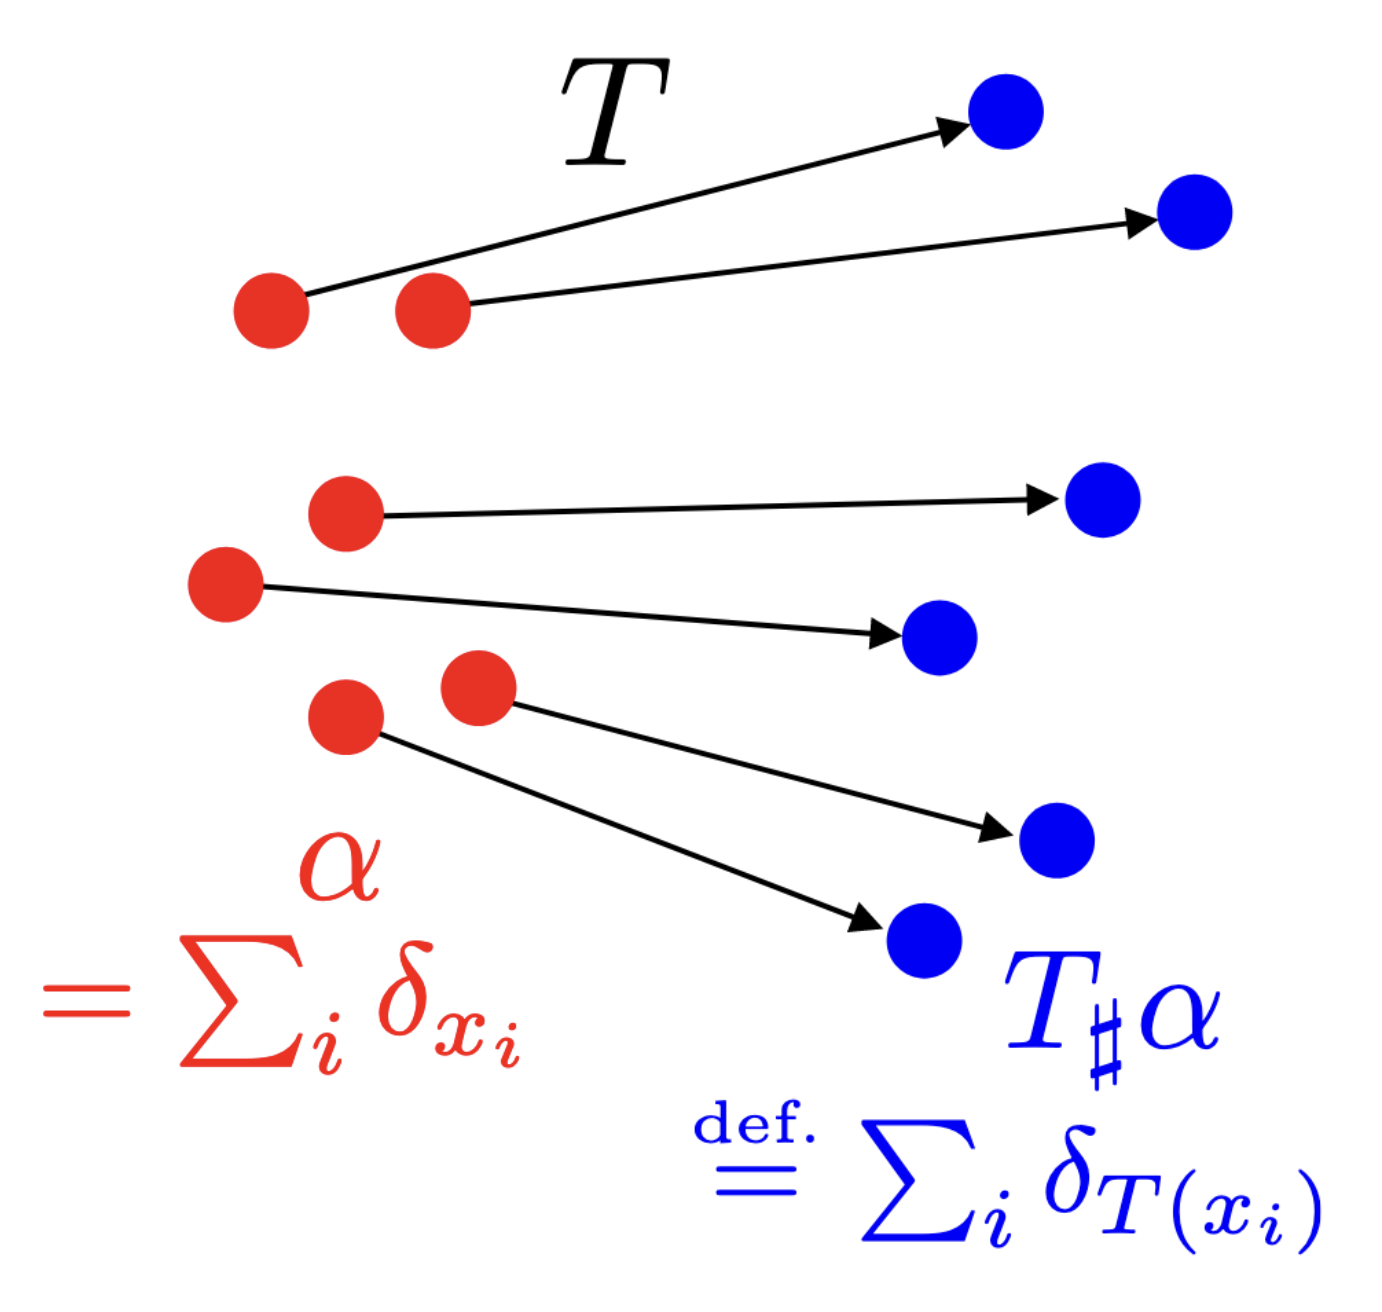
\includegraphics[width=0.42\textwidth]{png/push-forward.png}
            \caption{push-forward of a discrete measure}
        \end{minipage}
    \end{figure}

    \pause
    \vspace{-1em}
    Given two probability measures $\mu$ on $\mX$ and $\nu$ on $\mY$, and a 
    cost function $c(x,y)$. 
    Optimal transport could be generally formulated as the 
    Monge problem:

    \vspace{-.2em}
    \begin{equation}
        \min_T\;\left\{\int_\mX c(x,T(x))\;d\mu(x) : T_\#\mu = \nu \right\}
    \end{equation}

    \vspace{-.5em}
    The Monge problem between discrete measures is 
    introduced by Monge\footfullcite{Monge1781}.
\end{frame}

\begin{frame}{The Kantorovich formulation}
    \footnotesize
    Here's another general formulation of OT, 
    we first recall the three main scenarios for OT.

    \begin{figure}
        \captionsetup{font=scriptsize}
        \centering
        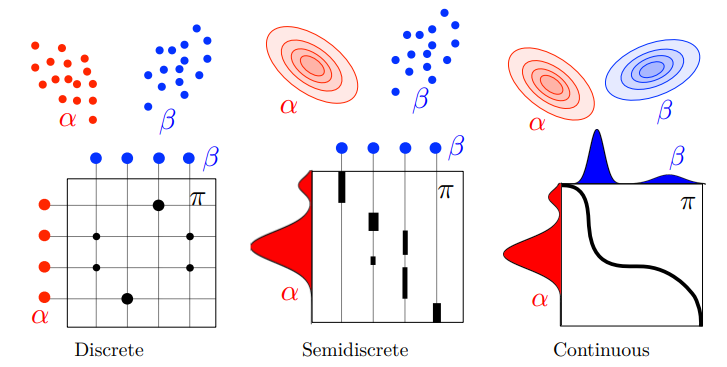
\includegraphics[width=0.6\textwidth]{png/3TypesOfOT.png}
    \end{figure}

    \pause
    Given two probability measures $\mu$ on $\mX$ and $\nu$ on $\mY$, and a 
    cost function $c(x,y)$. 
    Optimal transport could be generally formulated as
    the Kantorovich problem\footfullcite{Kantorovich1942}:
    \begin{equation}
        \mL_c(\mu,\nu)=\min_\pi \; \int_{\mX\times \mY} c(x,y) \;d\pi(x,y),
    \end{equation}
    where $\pi$ is a measure on $\mX\times \mY$, whose
    marginals are $\mu$ and $\nu$, that is,
    \begin{equation}
        \mu = \int_{\mY} \pi(\cdot, y) \;dy,\qquad 
        \nu = \int_{\mX} \pi(x, \cdot) \;dx.
    \end{equation}
\end{frame}

\begin{frame}{Wasserstein disrtance}
    \footnotesize
    Here we suppose $\mX=\mY$ and $c(x,y)=d(x,y)^p\;(p>1)$, where $d$ is a distance on $\mX$.

    \pause
    \begin{Thm}[Wasserstein distance]
        Under the above assumptions, $\mL_c(\mu,\nu)^{1/p}$ is a distance on $\pbms$.
    \end{Thm}

    The distance $\wass_p(\mu,\nu):=\mL_c(\mu,\nu)^{1/p}$ is called $p$-Wasserstein distance.

    \pause

    \begin{Def}[weak convergence]
        Suppose $\mX$ is compact. Say $(\mu_k)_{k\geq 1}\subset \pbms$ converges
        weakly to $\mu\in\pbms$ if
        \begin{equation}
            \int_{\mX} g\;d\mu_k \to \int_{\mX}g\;d\mu,\quad \forall g\in\cfun.
        \end{equation}
    \end{Def}

    \begin{Thm}[Wasserstein distance and weak convergence\footfullcite{Villani2009}]
        On a compact domain $\mX$, $(\mu_k)_{k\geq 1}\subset \pbms$ converges 
        weakly to $\mu\in\pbms$ if and only if $\wass_p(\mu_k,\nu)\to 0$.
    \end{Thm}
\end{frame}

\begin{frame}{Equivalence between the Kantorovich and Monge problems}
    \scriptsize
    \begin{Thm}[Kantorovich dual problem]
        The Kantorovich problem can be solved in the dual space by

        \vspace{-.7em}
        \begin{equation}
            \mL_c(\mu,\nu)=\sup_{(f,g)\in \mathcal{R}(c)} 
            \int_\mX f(x)\;d\mu(x) + \int_\mY g(y)\;d\nu(y),
            \label{equ:KantorovichDual}
        \end{equation}

        \vspace{-.4em}
        where the set of admissible dual potential is

        \vspace{-.4em}
        \begin{equation}
            \mathcal{R}(c) := \{(f,g) \in \cfun\times\cfuny : 
            \forall (x,y), f(x)+g(y)\leq c(x,y)\}.
        \end{equation}

        \vspace{-.4em}
        The pair $(f,g)$ is called Kantorovich potentials.
    \end{Thm}

    \pause
    \begin{Thm}[Brenier]
        In the case $\mX=\mY=\R^d$ and $c(x, y) =\|x-y\|_2^2$, 
        if at least one of the two input measures (denoted $\mu$) 
        has a density $\rho_\mu$ with respect to the Lebesgue measure, 
        then the optimal $\pi$ in the Kantorovich formulation is unique 
        and is supported on the graph $(x, T (x))$ of a Monge map
        $T : \R^d \to \R^d$. This means that $\pi = (\text{Id}, T)_\#\mu$, 
        i.e.

        \vspace{-.4em}
        \begin{equation}
            \int_{\mX\times \mY} h(x,y)\;d\pi(x,y)=\int_\mX h(x,T(x))\;d\mu(x),
            \quad \forall h\in\mathcal{C}(\mX\times \mY).
        \end{equation}

        \vspace{-.4em}
        Furthermore, this map $T$ is uniquely defined as the gradient 
        of a convex function $\varphi$, $T (x) = \nabla \varphi(x)$, 
        where $\varphi$ is the unique (up to an additive constant) convex 
        function such that $(\nabla\varphi)_\#\mu = \nu$. This convex 
        function is related to the dual potential $f$ solving 
        $(10)$ as

        \vspace{-.4em}
        \begin{equation}
            \varphi(x)=\frac{\| x\|_2^2}{2} - f(x).
        \end{equation}
    \end{Thm}
\end{frame}

\begin{frame}{1-D case}
\end{frame}

\begin{frame}
    \begin{center}
        {\Huge\calligra Thank You}
    \end{center}
\end{frame}

\end{document}